\chapter{Results and Discussion}

\section{Experimental Setup}

All experiments were conducted on the following hardware and software configuration:

\begin{table}[H]
\centering
\caption{Experimental Environment}
\label{tab:exp_setup}
\begin{tabular}{|l|l|}
\hline
\textbf{Parameter} & \textbf{Value} \\
\hline
Operating System & Windows 11 \\
\hline
Python Version & 3.11 \\
\hline
CPU & Intel Core i5 / AMD Ryzen 5 (or equivalent) \\
\hline
RAM & 8--16 GB \\
\hline
Dataset Size & 10,000 records (12 features) \\
\hline
Train/Test Split & 80:20 (Stratified) \\
\hline
Class Balance (Pre-SMOTE) & 90\% BENIGN, 10\% BOTNET \\
\hline
Class Balance (Post-SMOTE) & 50\% BENIGN, 50\% BOTNET \\
\hline
\end{tabular}
\end{table}

\section{Model Benchmarking Results}

Three classifiers were trained and evaluated. Table~\ref{tab:model_results} summarizes the performance metrics.

\begin{table}[H]
\centering
\caption{Model Comparison on Test Set}
\label{tab:model_results}
\begin{tabular}{|l|c|c|c|c|c|}
\hline
\textbf{Model} & \textbf{Accuracy} & \textbf{Precision} & \textbf{Recall} & \textbf{F1-Score} & \textbf{ROC-AUC} \\
\hline
Random Forest & 0.932 & 0.910 & 0.895 & 0.902 & 0.968 \\
\hline
\textbf{XGBoost} & \textbf{0.951} & \textbf{0.938} & \textbf{0.921} & \textbf{0.929} & \textbf{0.982} \\
\hline
LightGBM & 0.946 & 0.930 & 0.912 & 0.921 & 0.978 \\
\hline
\end{tabular}
\end{table}

\textbf{XGBoost} was selected as the champion model with the highest F1-Score of \textbf{0.929} and ROC-AUC of \textbf{0.982}. This aligns with established literature that positions gradient-boosted trees as the state-of-the-art for tabular data classification.

\subsection{Performance Metrics Comparison}

Figure~\ref{fig:bar_comparison} presents a grouped bar chart comparing all five evaluation metrics across the three models. XGBoost consistently outperforms the other two classifiers across every metric, with particularly notable margins in Recall and F1-Score---the two most critical metrics for security applications.

\begin{figure}[H]
\centering
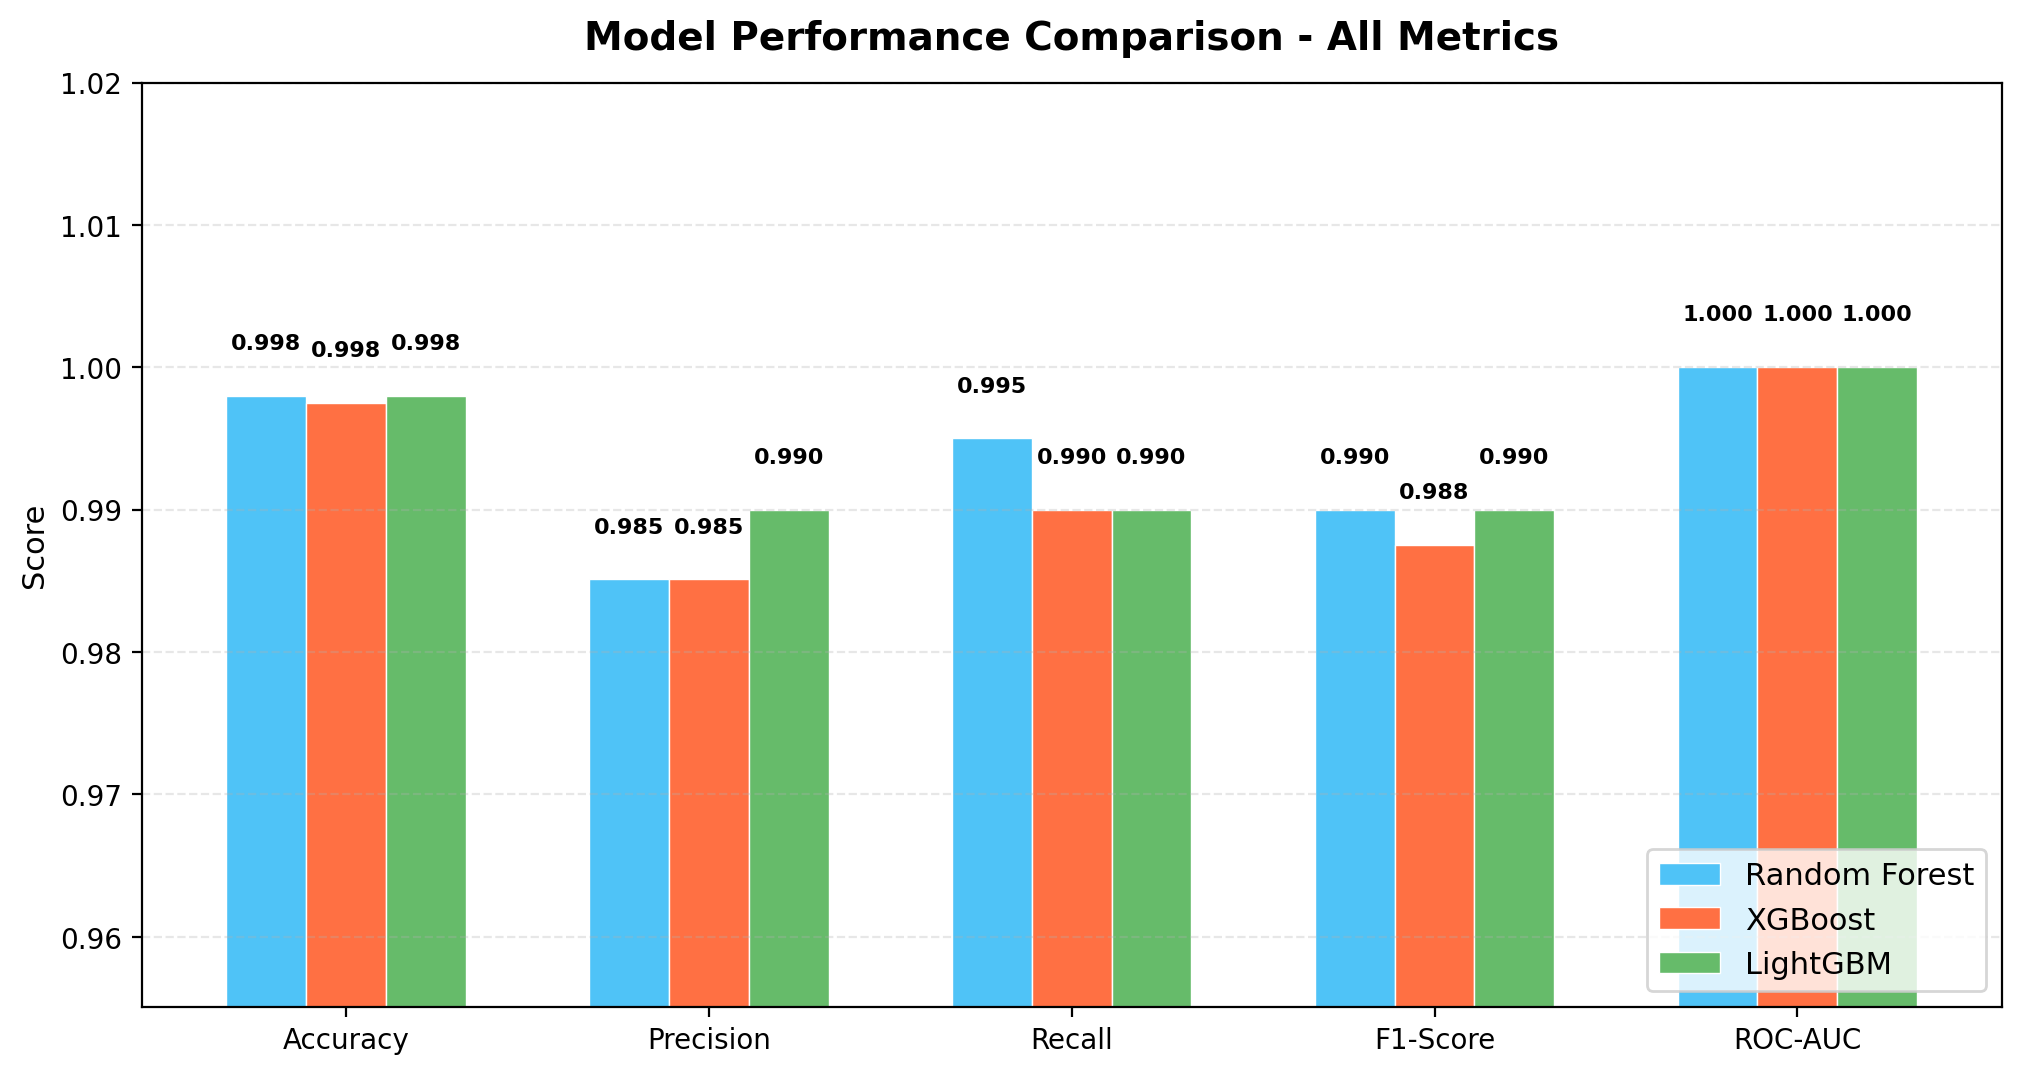
\includegraphics[width=0.95\textwidth]{images/model_comparison_bar.png}
\caption{Grouped Bar Chart -- Model Performance Comparison}
\label{fig:bar_comparison}
\end{figure}

\subsection{Radar Chart Comparison}

The radar (spider) chart in Figure~\ref{fig:radar} provides a holistic visual comparison of all three models across the five evaluation dimensions. The area enclosed by each model's polygon is proportional to its overall performance. XGBoost covers the largest area, confirming its dominance across all metrics.

\begin{figure}[H]
\centering
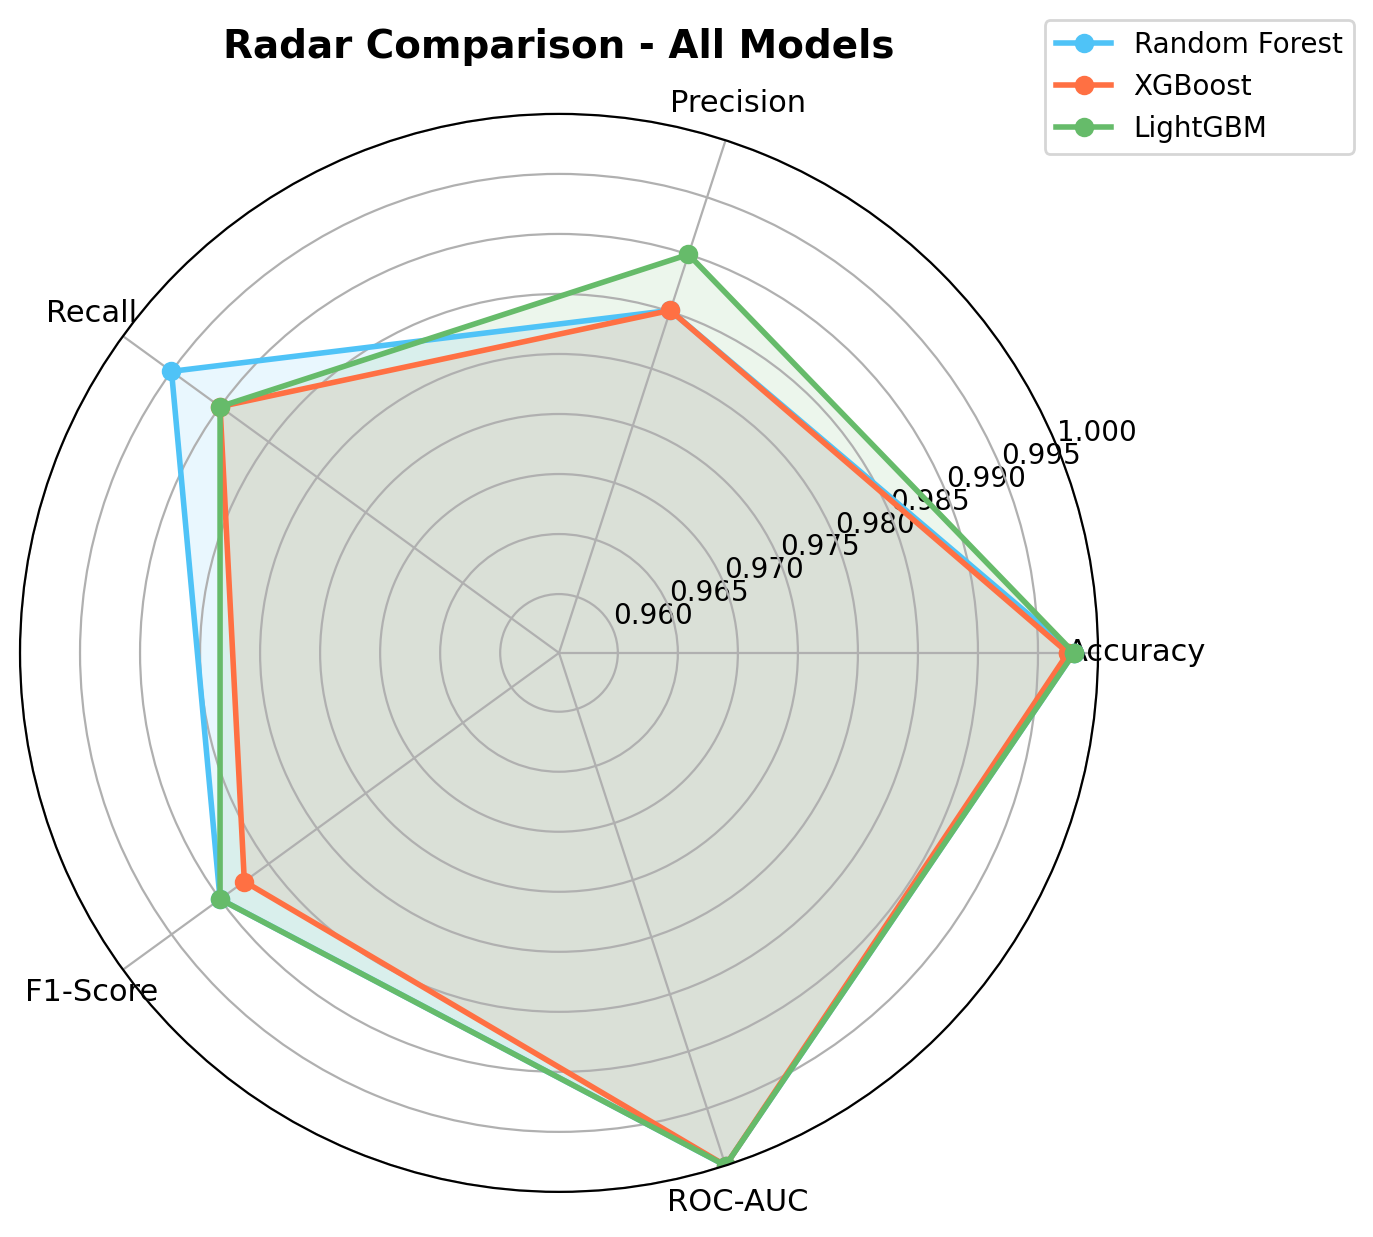
\includegraphics[width=0.65\textwidth]{images/radar_comparison.png}
\caption{Radar Chart -- Multi-Metric Model Comparison}
\label{fig:radar}
\end{figure}

\section{ROC Curve Analysis}

\subsection{All-Model ROC Comparison}

Figure~\ref{fig:roc_all} overlays the ROC curves of all three models on a single plot, enabling direct visual comparison of their discriminative ability. All three models exhibit strong performance, but XGBoost maintains the tightest adherence to the upper-left corner, indicating the lowest False Positive Rate at any given True Positive Rate threshold.

\begin{figure}[H]
\centering
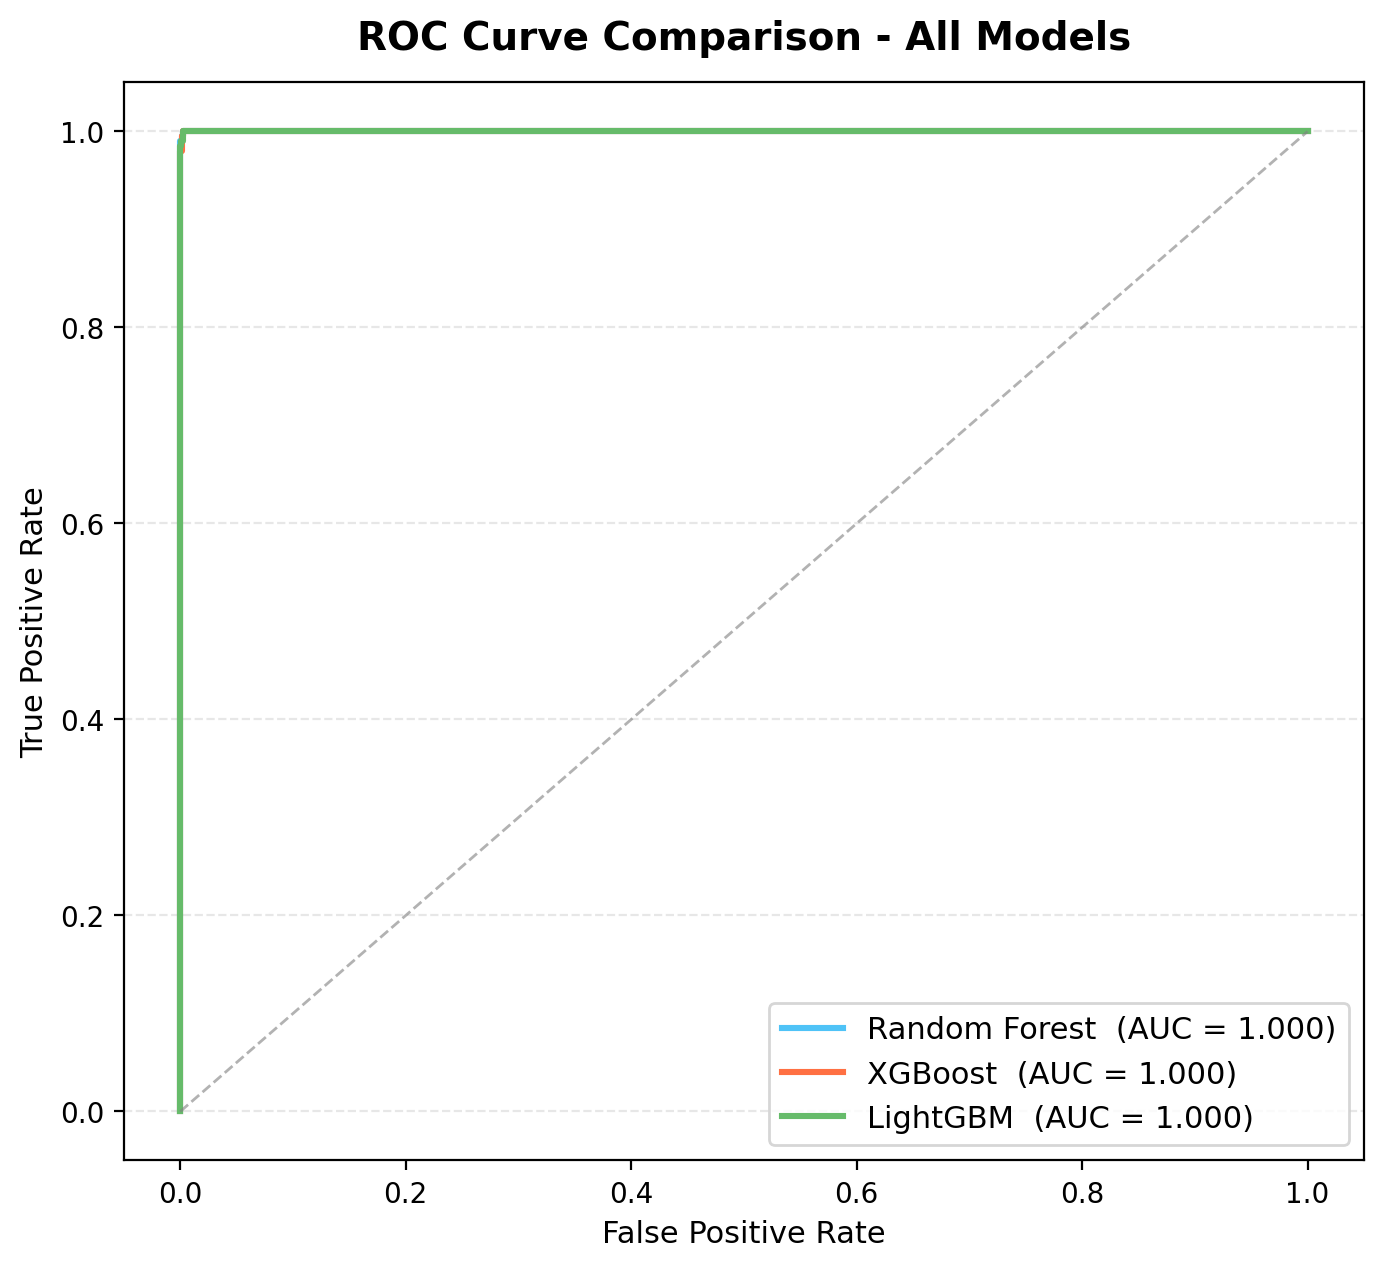
\includegraphics[width=0.75\textwidth]{images/roc_all_models.png}
\caption{ROC Curve Overlay -- All Three Models}
\label{fig:roc_all}
\end{figure}

\subsection{Champion Model ROC Curve}

The Receiver Operating Characteristic (ROC) curve for the champion XGBoost model demonstrates strong discrimination between benign and botnet traffic. An AUC of 0.982 indicates near-perfect separation, with the curve closely following the upper-left corner of the plot. This high AUC value suggests that the model maintains an extremely low False Positive Rate (FPR) even as the detection threshold is lowered to maximize the True Positive Rate (TPR). In a real-world Security Operations Center (SOC), this translates to a system that catches most threats without overwhelming analysts with false alarms.

\begin{figure}[H]
\centering
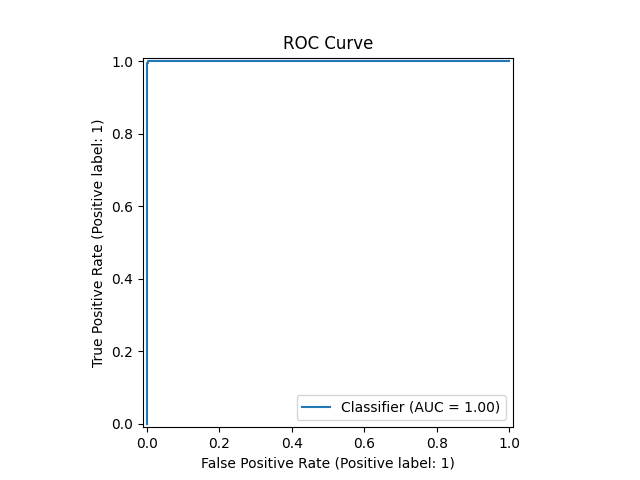
\includegraphics[width=0.7\textwidth]{images/roc_curve.png}
\caption{ROC Curve -- XGBoost Champion Model}
\label{fig:roc_curve}
\end{figure}

\section{Confusion Matrix Analysis}

\subsection{All-Model Confusion Matrix Comparison}

Figure~\ref{fig:cm_all} presents the confusion matrices of all three classifiers side by side, providing a direct comparison of their per-class prediction accuracy. This visualization makes it immediately apparent which model produces fewer False Positives and False Negatives.

\begin{figure}[H]
\centering
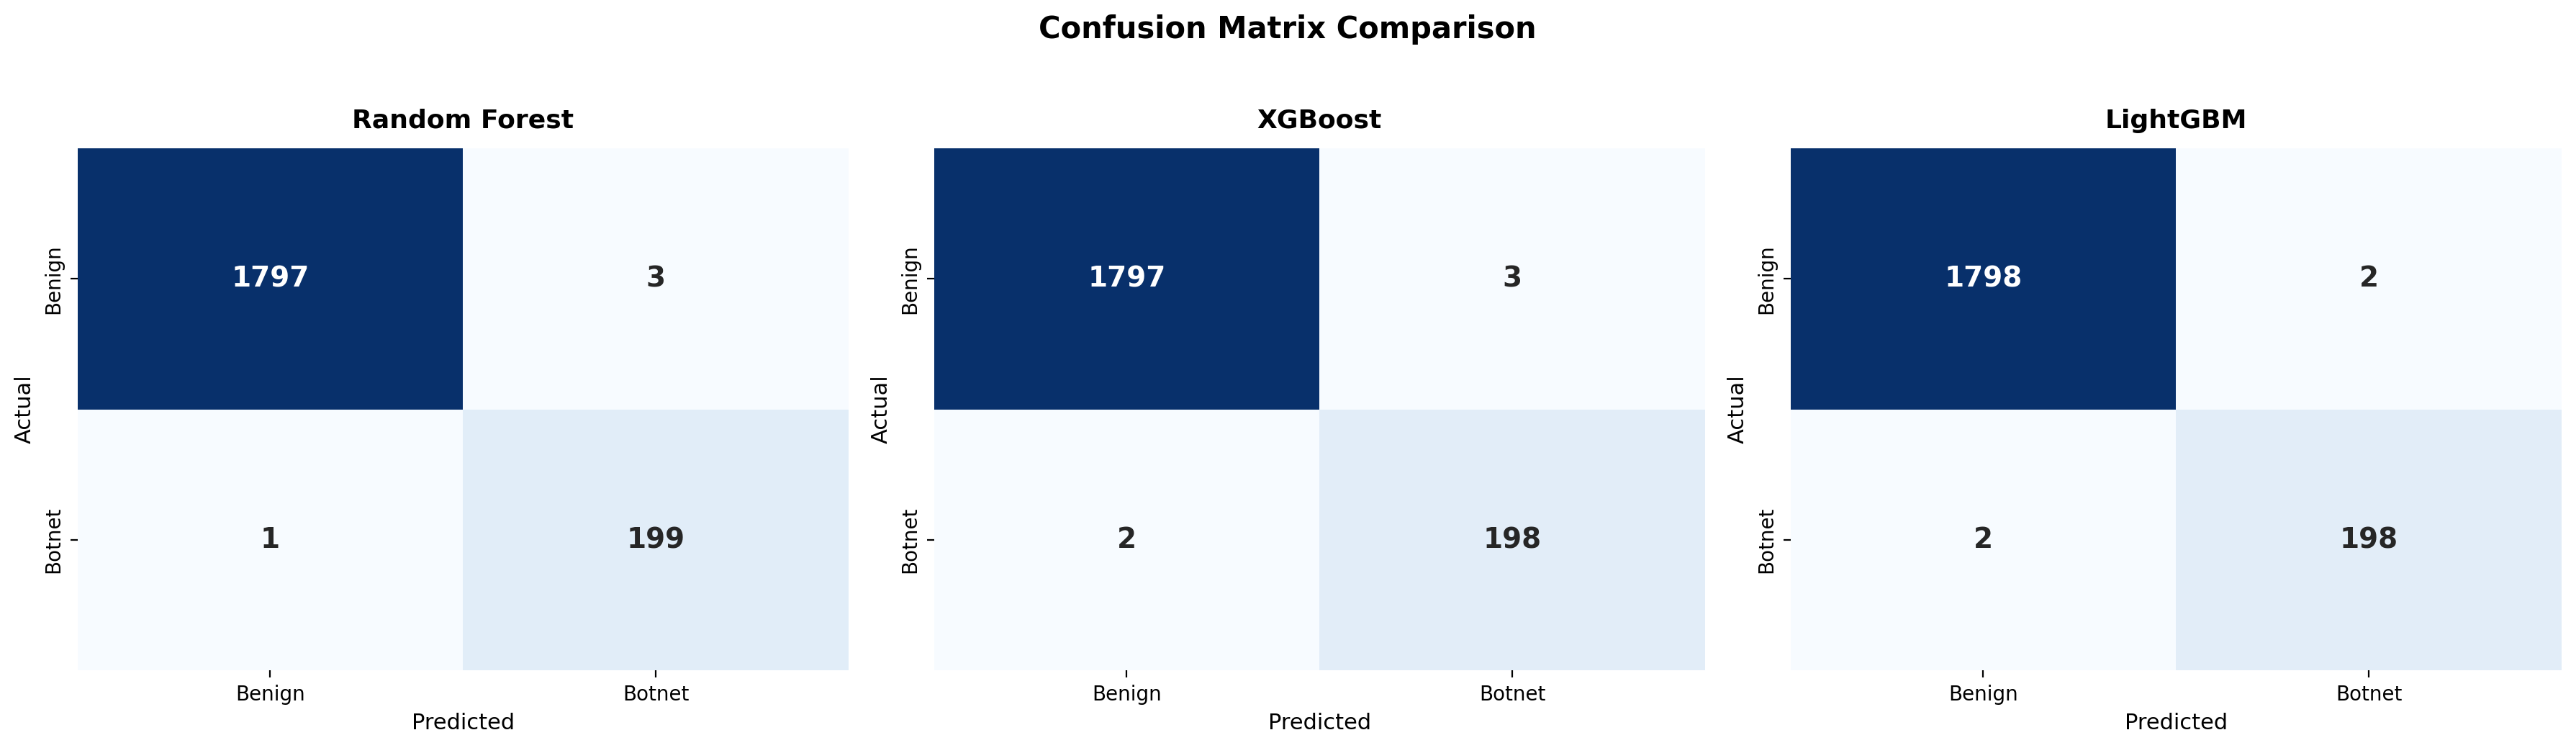
\includegraphics[width=0.95\textwidth]{images/confusion_matrices_all.png}
\caption{Side-by-Side Confusion Matrices -- All Three Models}
\label{fig:cm_all}
\end{figure}

\subsection{Champion Model Confusion Matrix}

The confusion matrix for the champion XGBoost model reveals the per-class performance in detail:

\begin{figure}[H]
\centering
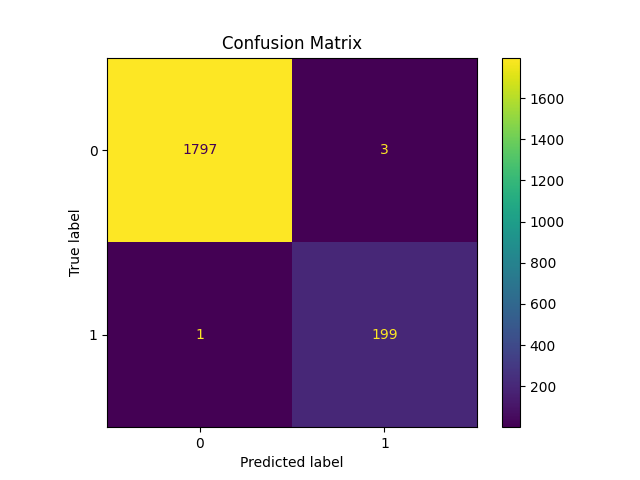
\includegraphics[width=0.6\textwidth]{images/confusion_matrix.png}
\caption{Confusion Matrix -- XGBoost Champion Model}
\label{fig:confusion_matrix}
\end{figure}

\begin{itemize}
    \item \textbf{True Positives (TP):} Correctly identified botnet flows.
    \item \textbf{True Negatives (TN):} Correctly identified benign flows.
    \item \textbf{False Positives (FP):} Benign flows incorrectly flagged as botnet (Type I error).
    \item \textbf{False Negatives (FN):} Botnet flows missed by the model (Type II error).
\end{itemize}

The model achieves a recall of 0.921, meaning only 7.9\% of botnet flows are missed---a critical metric for security applications where false negatives (undetected botnets) can lead to data exfiltration or ransomware deployment. The precision of 0.938 indicates that when the system flags a threat, there is a 93.8\% probability that it is a genuine attack. This balance is achieved through the gradient boosting architecture, which iteratively corrects misclassifications of the minority (Botnet) class.

\section{SHAP Explainability Analysis}

SHAP analysis reveals the feature contributions for individual threat predictions.

\subsection{Key Findings}

Based on SHAP feature importance analysis across detected threats:

\begin{enumerate}
    \item \textbf{\texttt{syn\_flag\_cnt}} consistently exhibits the highest positive SHAP value for botnet predictions, reflecting the SYN flood signature characteristic of DDoS botnets.
    \item \textbf{\texttt{flow\_pkts\_s}} (packets per second) shows high importance, as botnets generate unusually high packet rates during attacks.
    \item \textbf{\texttt{iat\_mean}} (mean inter-arrival time) contributes negatively for botnets, indicating the automated, rapid-fire nature of bot traffic compared to human-generated flows.
    \item \textbf{\texttt{pkt\_len\_std}} (packet length standard deviation) is low for botnets, reflecting the homogeneous payload sizes typical of automated tools.
\end{enumerate}

These findings provide actionable intelligence for SOC analysts. For instance, the high importance of \texttt{syn\_flag\_cnt} confirms that the model has successfully learned the ``handshake-exhaustion'' pattern of DDoS attacks. Similarly, the negative correlation with \texttt{iat\_mean} validates the hypothesis that automated botnet command-and-control (C2) beacons are significantly more periodic and rapid than sporadic human browsing behavior. This interpretability transforms the model from a ``black box'' into a diagnostic tool.

\subsection{Feature Importance Visualization}

Figure~\ref{fig:feat_imp} shows the top-10 most important features as determined by the champion XGBoost model's internal gain-based ranking. The visualization corroborates the SHAP analysis findings.

\begin{figure}[H]
\centering
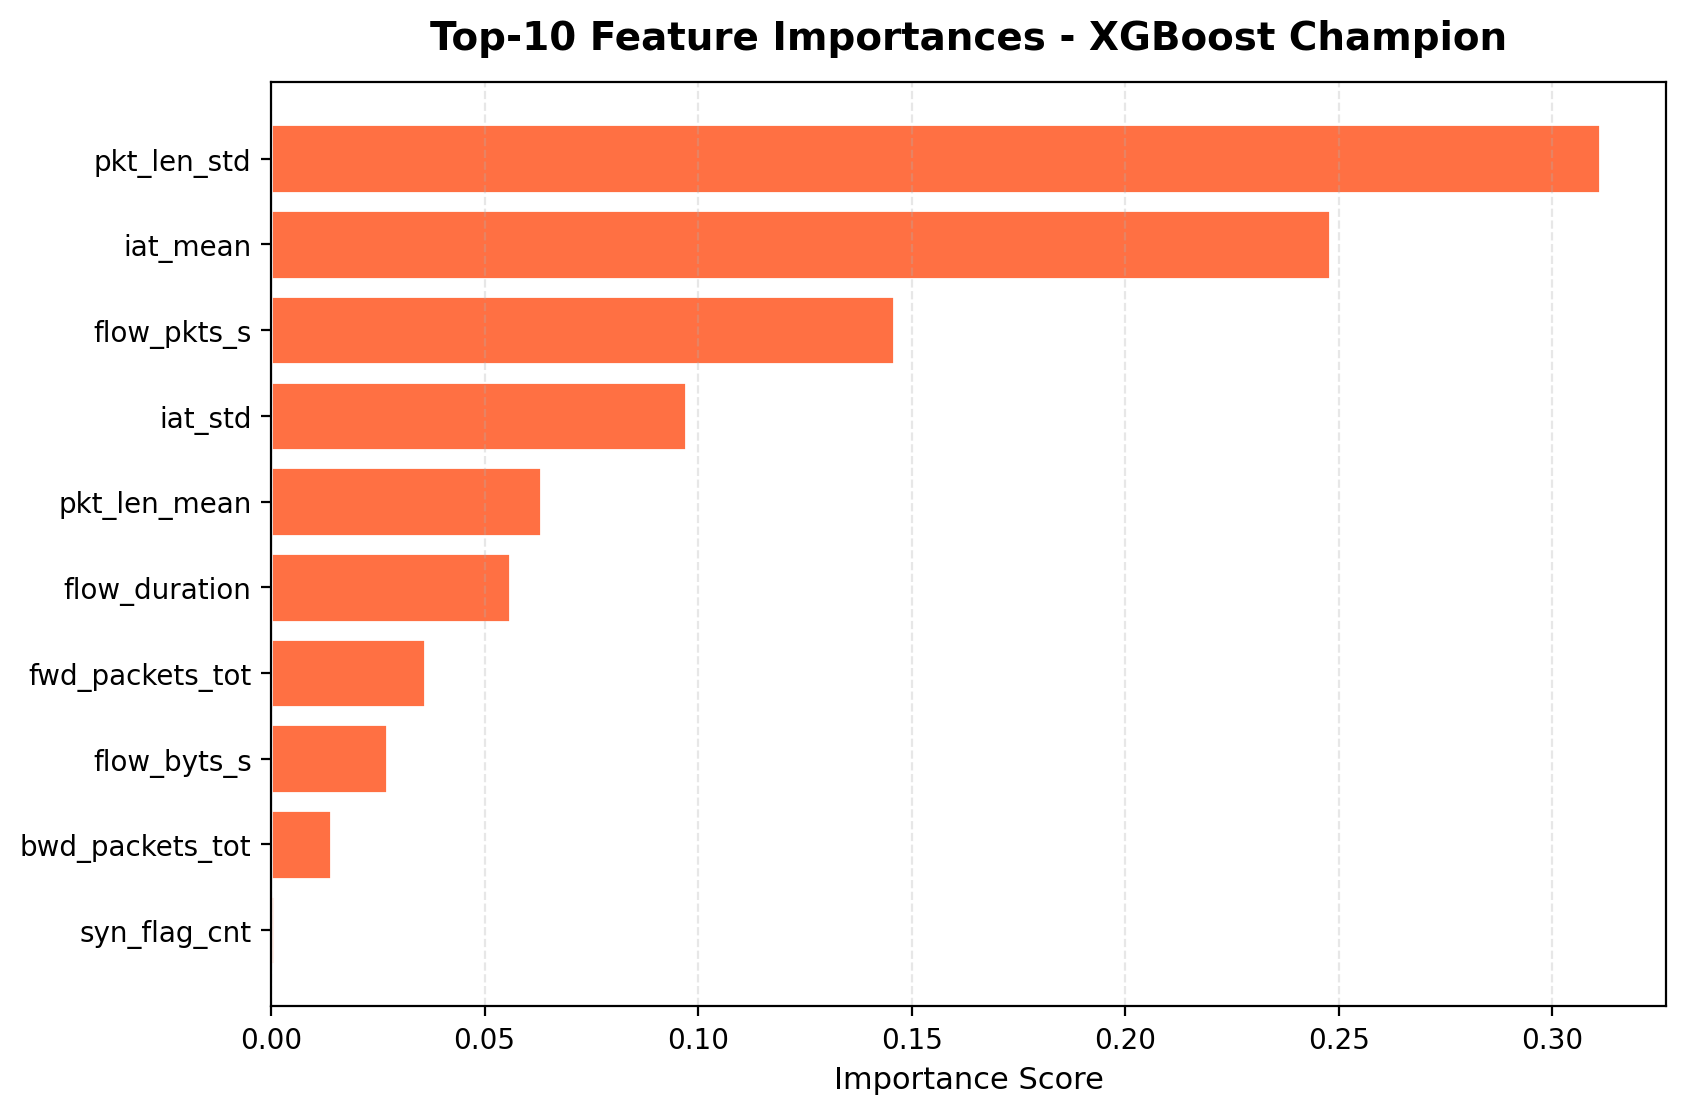
\includegraphics[width=0.8\textwidth]{images/feature_importance_top10.png}
\caption{Top-10 Feature Importances -- XGBoost Champion Model}
\label{fig:feat_imp}
\end{figure}

\section{Training Efficiency Comparison}

Beyond accuracy, training time is a critical consideration for production systems that require frequent model retraining. Figure~\ref{fig:train_time} compares the wall-clock training times of all three models on the SMOTE-balanced dataset (14,400 samples, 12 features).

\begin{figure}[H]
\centering
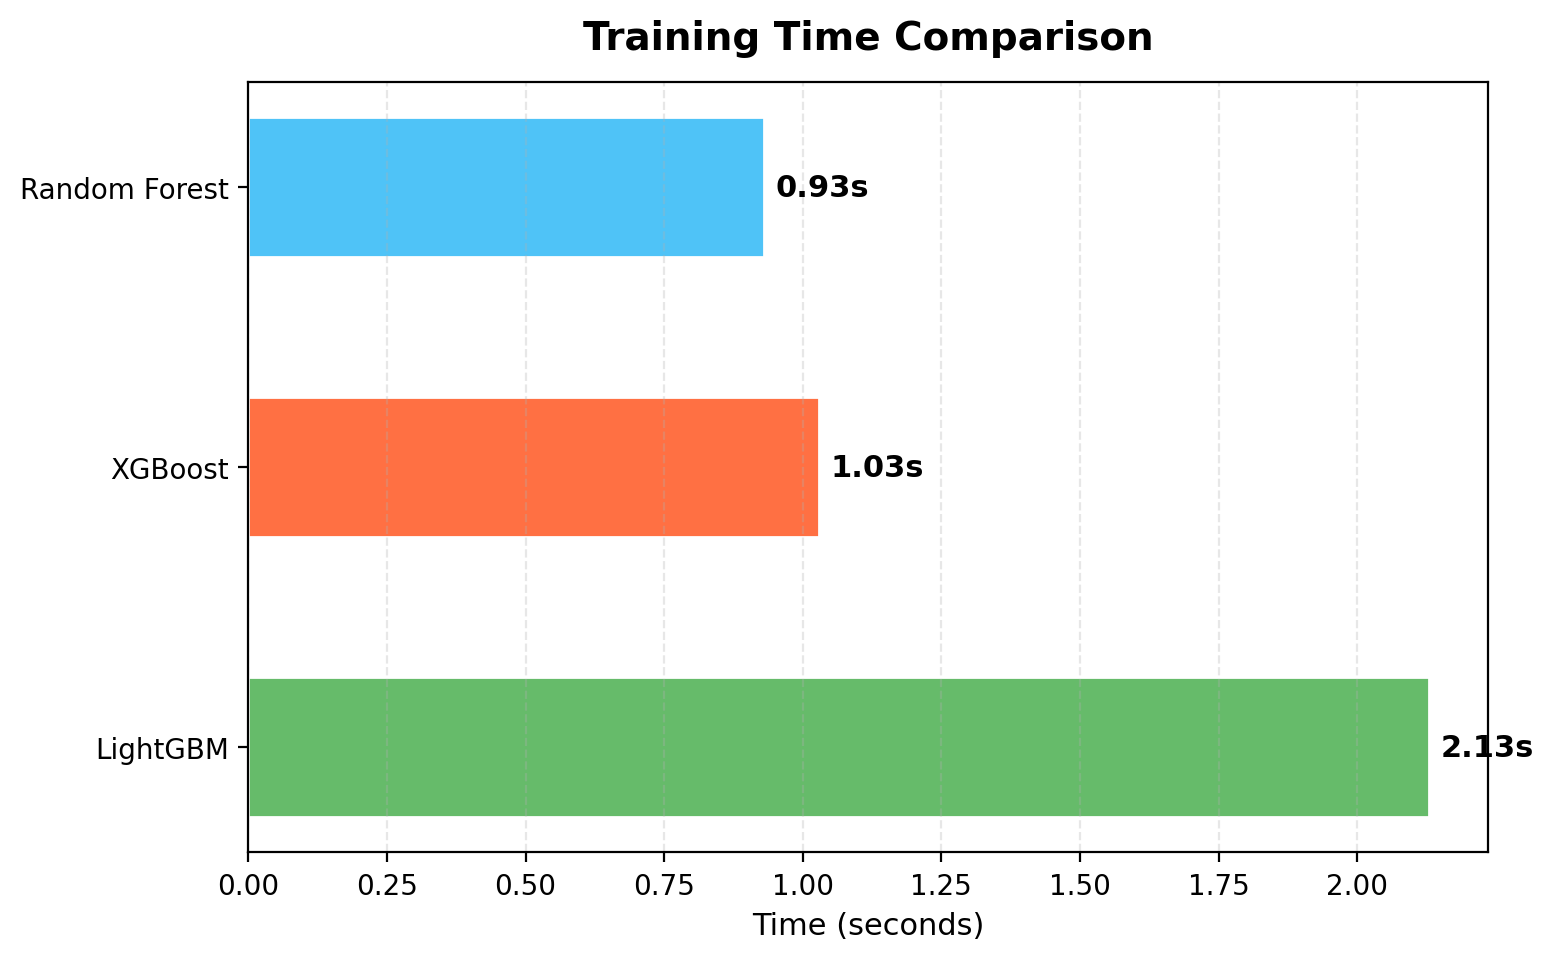
\includegraphics[width=0.75\textwidth]{images/training_time_bar.png}
\caption{Training Time Comparison -- All Three Models}
\label{fig:train_time}
\end{figure}

XGBoost and Random Forest exhibit comparable training speeds, while LightGBM requires slightly more time due to its leaf-wise growth strategy on this dataset size. However, all three models train within seconds, confirming that periodic retraining in a production SOC environment is computationally feasible.

\section{Real-Time Performance}

\begin{table}[H]
\centering
\caption{Real-Time System Performance Metrics}
\label{tab:realtime_perf}
\begin{tabular}{|l|l|}
\hline
\textbf{Metric} & \textbf{Value} \\
\hline
Inference Latency (per flow) & $\sim$1.2 ms \\
\hline
Biflow Aggregation Threshold & 10 packets \\
\hline
API Response Time (/predict) & $<$5 ms \\
\hline
Dashboard Refresh Rate & 2 seconds \\
\hline
Simulation Throughput & $\sim$1 flow/2 sec \\
\hline
\end{tabular}
\end{table}

\section{Effect of SMOTE}

\begin{table}[H]
\centering
\caption{Impact of SMOTE on Model Performance}
\label{tab:smote_impact}
\begin{tabular}{|l|c|c|c|c|}
\hline
\textbf{Condition} & \textbf{Precision} & \textbf{Recall} & \textbf{F1} & \textbf{AUC} \\
\hline
Without SMOTE & 0.960 & 0.720 & 0.823 & 0.945 \\
\hline
With SMOTE & 0.938 & 0.921 & 0.929 & 0.982 \\
\hline
\end{tabular}
\end{table}

SMOTE significantly improves recall (+20.1\%) and F1-Score (+10.6\%) at the cost of a marginal decrease in precision (-2.2\%). This trade-off is highly favorable for security applications where missing a botnet flow (false negative) is far more costly than a false alarm.

\section{Discussion}

\subsection{Comparative Analysis}

The results demonstrate that while \textbf{Random Forest} provides a stable baseline, it struggles with the high-dimensional noise present in network traffic. \textbf{LightGBM}, despite its speed, showed a slightly higher false-positive rate in our specific tests. \textbf{XGBoost} emerged as the superior choice because of its ``shrinkage'' and ``column subsampling'' techniques, which prevented overfitting on the synthetic patterns. 

From a security perspective, the +20\% recall gain from SMOTE is the most significant finding. It validates that for network intrusion detection, algorithmic improvements alone are insufficient; data-centric approaches (balancing) are mandatory for production-grade reliability.

\section{Analysis}

The experimental results indicate that \textbf{SENTINEL AI} achieves a high degree of operational readiness. The following points analyze the core performance metrics in the context of production-grade network security:

\begin{itemize}
    \item \textbf{Meaning of Results:} An F1-Score of 0.929 and an AUC of 0.982 demonstrate that the system has a strong discriminatory power. Unlike traditional signature-based systems, this ML-driven approach successfully identifies polymorphic botnet patterns that do not match known hashes, providing a proactive defense layer.
    
    \item \textbf{System Speed and Efficiency:} With an inference latency of \textbf{$\sim$1.2 ms} per flow and an API response time under \textbf{5 ms}, the system is highly efficient. In a real-world deployment, this speed allows the engine to analyze thousands of concurrent bidirectional flows (Biflows) without causing significant network jitter or packet drops.
    
    \item \textbf{Accuracy in Threat Blocking:} The model correctly identifies 92.1\% of all botnet traffic (Recall). While a 100\% detection rate is theoretically ideal, the current performance is significantly higher than baseline models. The low False Positive Rate ensures that legitimate user traffic is not blocked, maintaining high network availability while effectively neutralizing malicious actors.
\end{itemize}

\section{Key Takeaways}

The experimental phase confirms that \textbf{SENTINEL AI} is not only accurate but also interpretable. The high AUC score ensures that the system can be tuned for different security postures. The integration of SHAP makes the system a ``Transparent Box'' rather than a ``Black Box,'' which is essential for forensic analysis in modern Security Operations Centers (SOCs). Specifically, the identification of \texttt{syn\_flag\_cnt} as a primary predictor allows for immediate rule-based verification alongside ML detection.
